\chapter{Redes neuronales}\label{Chapter7} 
% chktex-file 8
% chktex-file 12
% chktex-file 13
% chktex-file 44

Veremos redes neuronales poco profundas (no más de 2 capas ocultas). La idea básica es transformar un conjunto de variables capa a capa hasta llegar a un conjunto de variables fácilmente separables o ``regresables'' por la ultima capa. El resultado del pesado se pasa por una funcion de activacion no lineal. El peso $w_{ij}$ conecta la neurona j de la capa l con la neurona i de la capa l+1. No contamos el bias como neurona, asiq ue en el ejemplo que pone hay 3. El bias es un vector siempre, con dimension $\text{neuronas en esa capa} \times 1$. PAra el caso de la capa de entrada, la activacion es directametne la entrada. 

\section{Introducción}

Consideremos un problema de aprendizaje supervisado donde tenemos acceso a ejemplos de entrenamiento etiquetados $(x^{(i)}, y^{(i)})$. Las redes neuronales ofrecen una forma de definir una hipótesis compleja y no lineal $h_{W,b}(x)$, con parámetros $W, b$ que podemos ajustar a nuestros datos. \\

Para describir las redes neuronales, comenzaremos describiendo la red neuronal más simple posible, una que comprende una sola ``neurona''. Utilizaremos el diagrama \ref{fig:7.1} para denotar una sola neurona

\begin{figure}[H]
\centering
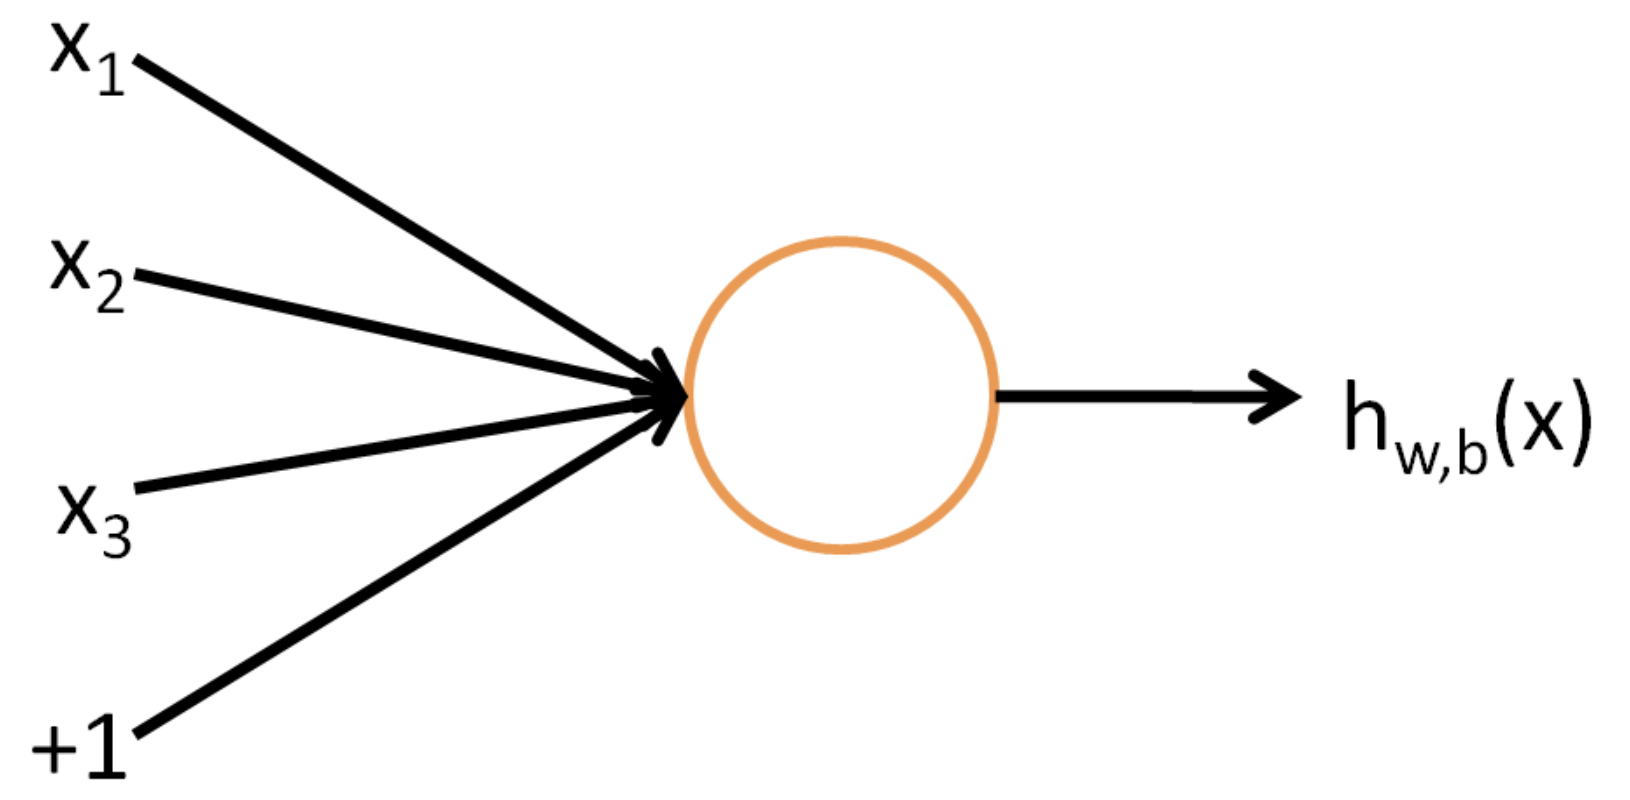
\includegraphics[width=0.4\textwidth]{fotos/40.png}
\caption{Diagrama de una neurona simple}
\label{fig:7.1}
\end{figure}

Esta ``neurona'' es una unidad computacional que toma como entrada $x_1, x_2, x_3$ (y un término de intercepto $+1$; este \textit{bias} no se cuenta como ``neurona''), y produce una salida 
\begin{equation}
h_{W,b}(x) = f(W^T x) = f\left(\sum_{i=1}^{3} W_i x_i + b\right)
\end{equation}

\noindent donde $f: \mathbb{R} \rightarrow \mathbb{R}$ se denomina función de activación. 

\subsection{Función de activación}

\subsubsection{Función sigmoide}

\noindent Aquí, elegiremos $f(\cdot)$ como la función sigmoide:
\begin{equation}
f(z) = \frac{1}{1 + e^{-z}}
\end{equation}

\noindent función acotada entre 0 y 1 también conocida como función logística estándar. Así, nuestra única neurona corresponde exactamente al mapeo de entrada-salida definido por la regresión logística. Una propiedad importante de esta función es que su derivada de puede escribir en términos de la misma función:
\begin{equation}
f'(z) = f(z)(1 - f(z))
\end{equation}

\begin{figure}[h]
\centering
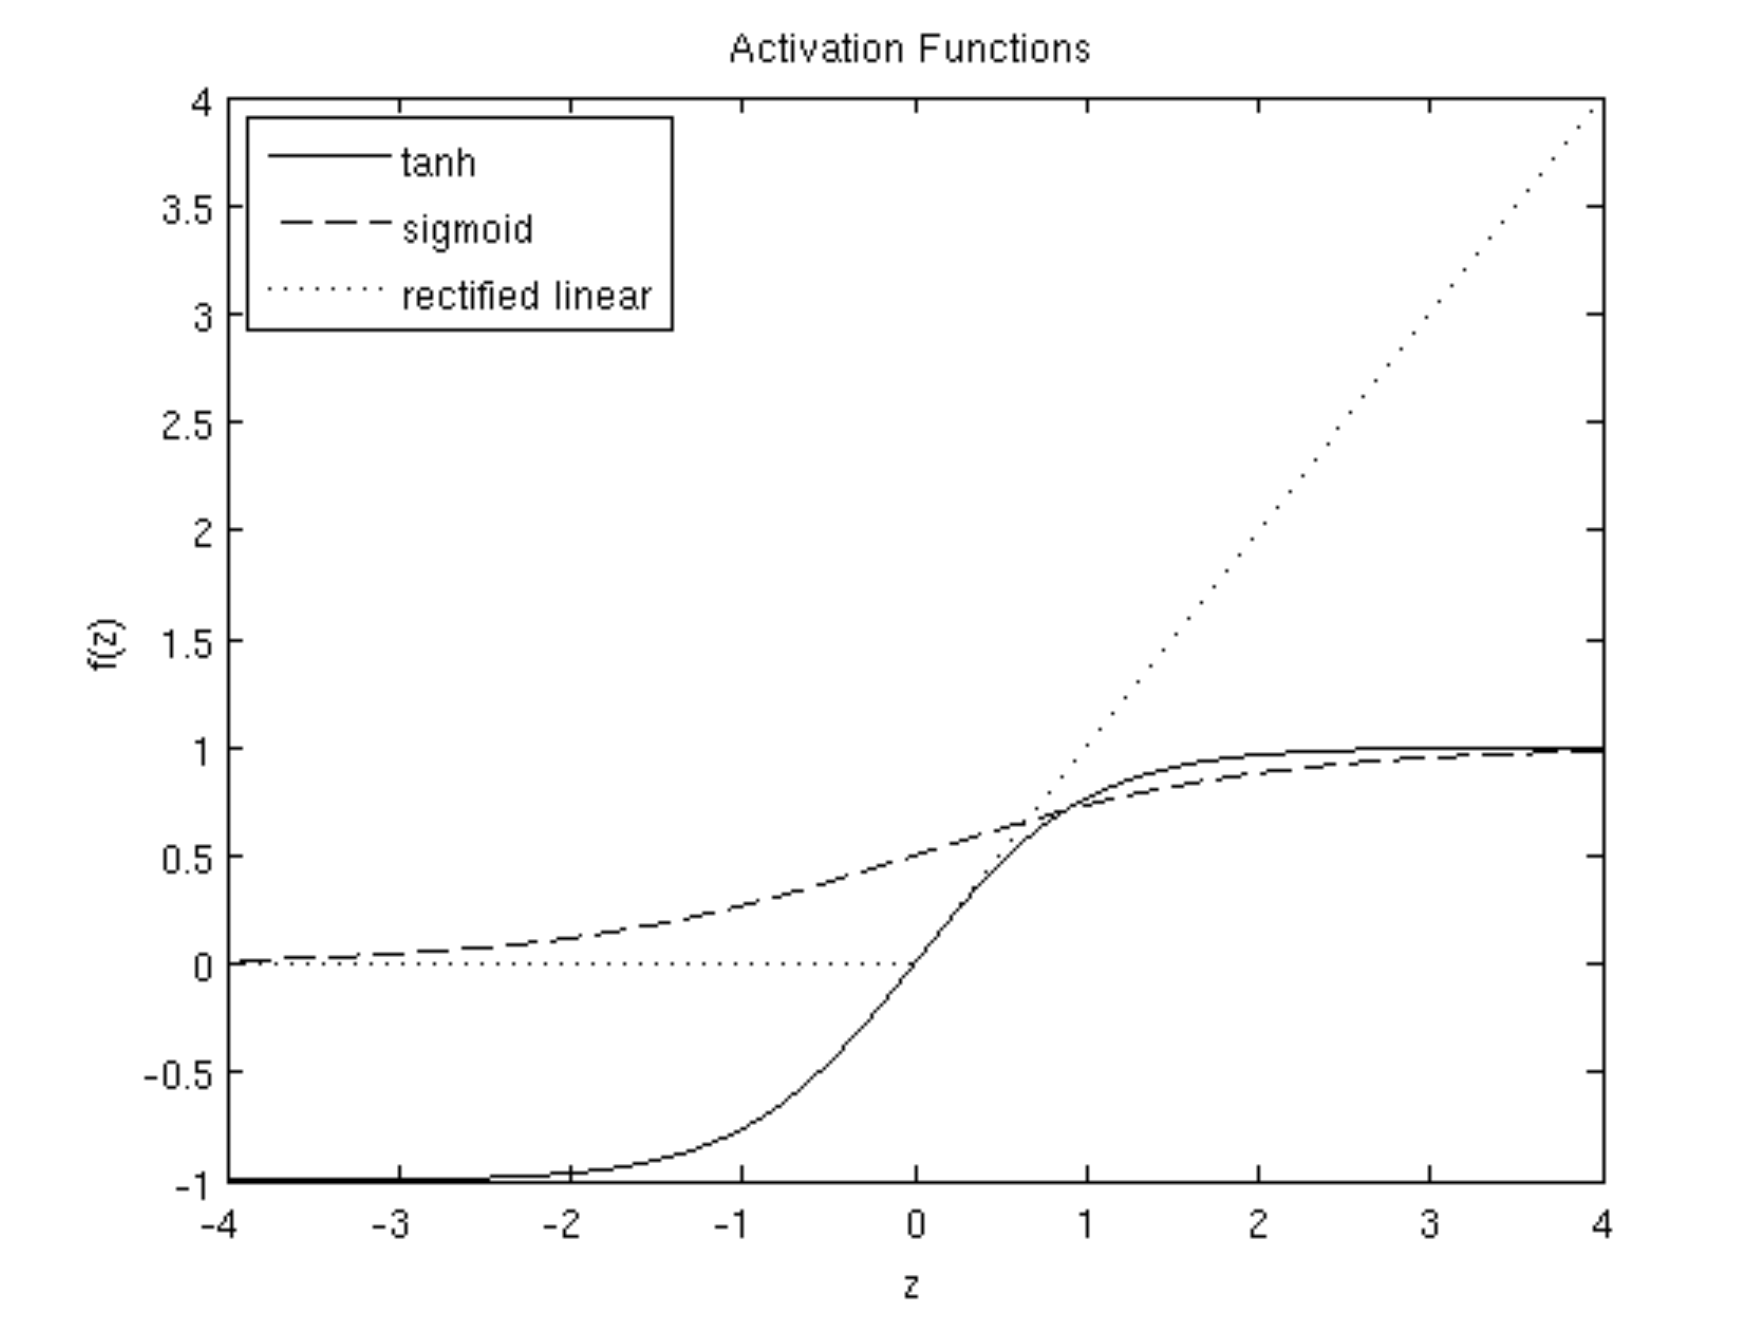
\includegraphics[width=0.6\textwidth]{fotos/41.png}
\caption{Funciones de activación: Sigmoide, tanh y ReLU}
\label{fig:7.2}
\end{figure}

\subsubsection{Tangente hiperbólica}

Aunque usaremos la función sigmoide, vale la pena notar que otra elección común para $f$ es la función tangente hiperbólica, o tanh:
\begin{equation}
f(z) = \tanh(z) = \frac{e^{z} - e^{-z}}{e^{z} + e^{-z}}
\end{equation}

La función $\tanh(z)$ es una versión reescalada de la sigmoide, y su rango de salida es $[-1, 1]$ en lugar de $[0,1]$. La derivada de esta función toma la forma $f'(z) = 1 - (f(z))^2$. 

\subsubsection{Función lineal rectificada ReLU}

Una función de activación diferente, la función lineal rectificada (ReLU), a menudo funciona mejor en la práctica para redes neuronales profundas. Esta función de activación es diferente de la sigmoide y la tanh porque no está acotada ni es continuamente diferenciable. La función de activación lineal rectificada se define como:
\begin{equation}
f(z) = \max(0, z)
\end{equation}

La función lineal rectificada es lineal por tramos y se satura exactamente en $0$ cuando la entrada $z$ es menor que $0$. Su derivada (gradiente) es 0 para $z<0$ y 1 para $z > 0$. El gradiente no está definido en $z = 0$, aunque esto no causa problemas en la práctica porque promediamos el gradiente sobre muchos ejemplos de entrenamiento durante la optimización.

\subsubsection{Funciones gaussianas de base radial}

El modelo de redes neuronales de funciones de base radial (RBF) es un modelo no lineal que utiliza funciones de base radial como funciones de activación. Las funciones de base radial son funciones que dependen solo de la distancia radial al origen, por lo que su valor es el mismo en todos los puntos que equidistan del origen. Sean matrices de covarianza cualesquiera, las funciones de base radial se definen como:
\begin{equation}
f_j(\mathbf{z}) = \exp\left\{-\frac{1}{2}(\mathbf{z} - \boldsymbol{\mu}_j)^T \boldsymbol{\Sigma}_j^{-1}(\mathbf{z} - \boldsymbol{\mu}_j)\right\}
\end{equation}

Como las matrices de covarianza son simétricas, se tiene que cada función de base radial tiene $d(d + 3)/2$ parámetros independientes ajustables, donde $d$ es la dimensión del espacio de entrada. \\


\section{Modelo de red neuronal}

Una red neuronal se construye conectando muchas ``neuronas'', de modo que la salida de una neurona puede ser la entrada de otra. Por ejemplo, la figura \ref{fig:7.3} muestra una pequeña red neuronal:

\begin{figure}[h]
\centering
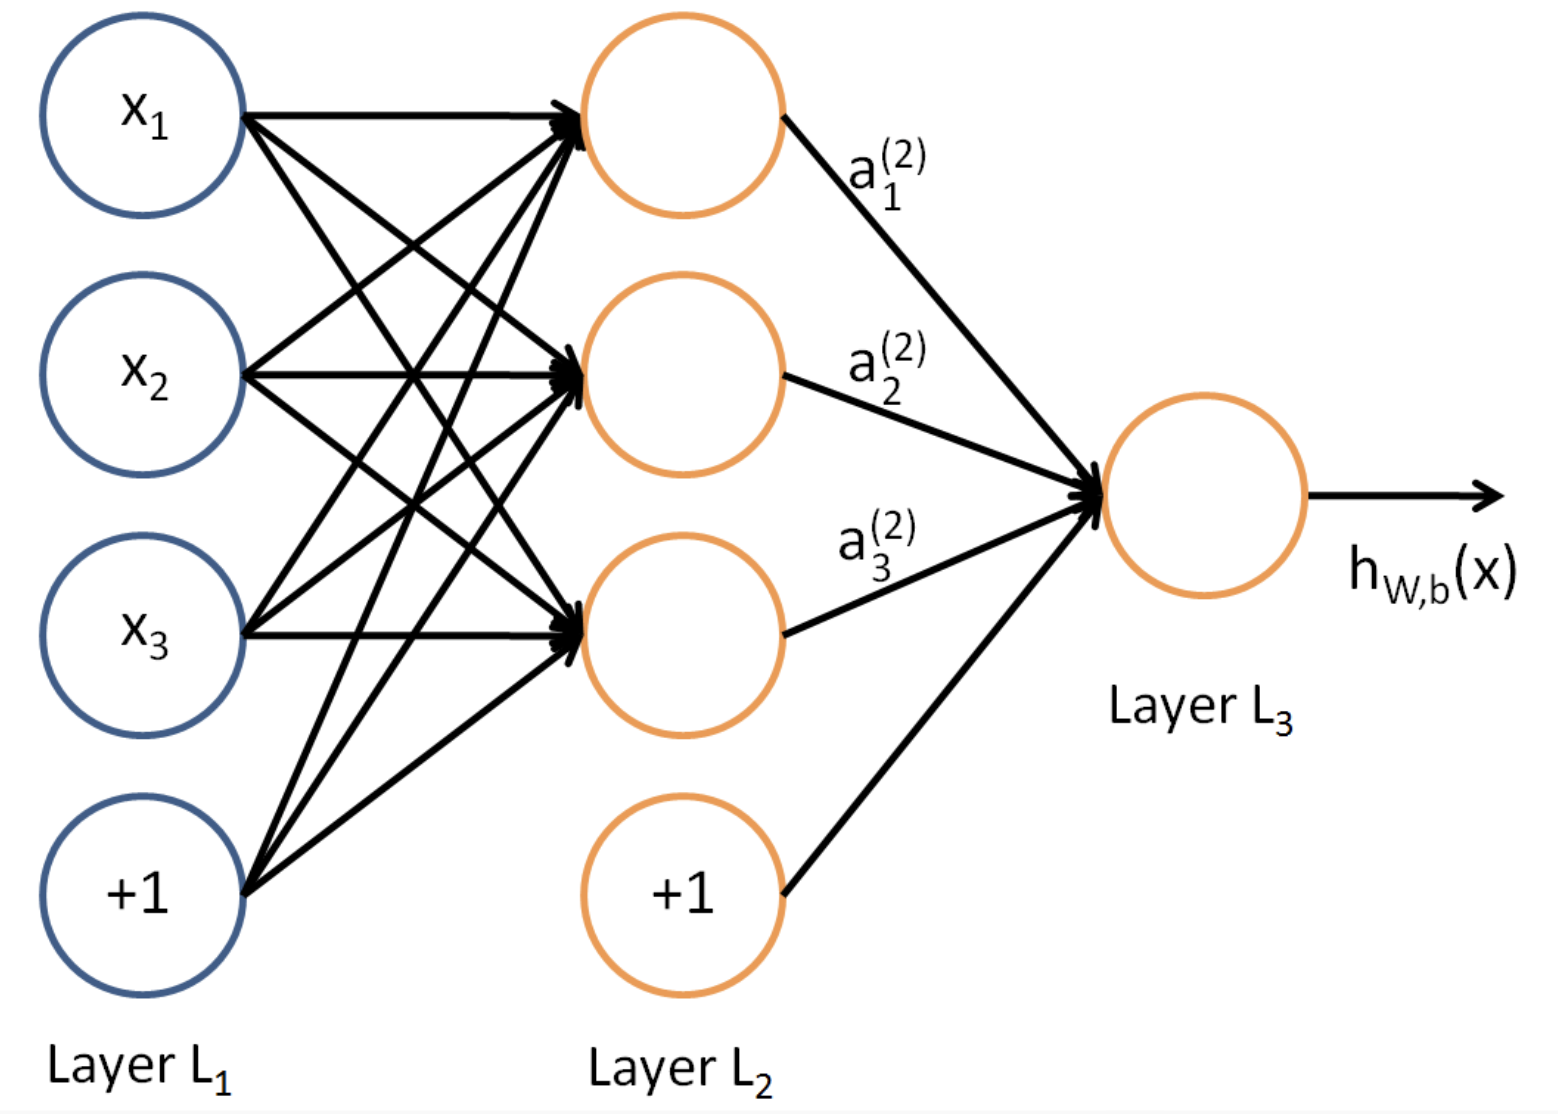
\includegraphics[width=0.5\textwidth]{fotos/42.png}
\caption{Ejemplo de una red neuronal pequeña}
\label{fig:7.3}
\end{figure}

En esta figura, hemos utilizado círculos para denotar también las entradas a la red. Los círculos etiquetados como ``+1'' se llaman unidades de sesgo y corresponden al término de intercepto. La capa más a la izquierda de la red se llama capa de entrada, y la capa más a la derecha la capa de salida (que, en este ejemplo, tiene solo una unidad). La capa intermedia de nodos se llama capa oculta, porque sus valores no se observan en el conjunto de entrenamiento. También decimos que nuestro ejemplo de red neuronal tiene 3 unidades de entrada (sin contar la unidad de sesgo), 3 unidades ocultas y 1 unidad de salida. \\

Denotaremos $n_l$ como el número de capas en nuestra red; por lo tanto, $n_l = 3$ en nuestro ejemplo. Etiquetamos la capa $l$ como $L_l$, por lo que la capa $L_1$ es la capa de entrada y la capa $L_{n_l}$ la capa de salida. \\

Nuestra red neuronal tiene parámetros $(W, b) = (W^{(1)}, b^{(1)}, W^{(2)}, b^{(2)})$, donde escribimos $W_{ij}^{(l)}$ para denotar el parámetro (o peso) asociado con la conexión entre la unidad $j$ en la capa $l$ y la unidad $i$ en la capa $l+1$ (nota el orden de los índices). Además, $b_i^{(l)}$ es el sesgo asociado con la unidad $i$ en la capa $l+1$. Así, en nuestro ejemplo, tenemos $W^{(1)} \in \mathbb{R}^{3 \times 3}$ y $W^{(2)} \in \mathbb{R}^{1 \times 3}$. Note que las unidades de sesgo no tienen entradas ni conexiones entrantes, ya que siempre sacan el valor $+1$; en nuestro ejemplo $b^{(1)} \in \mathbb{R}^{3 \times 1}$ y $b^{(2)} \in \mathbb{R}^{1 \times 1}$. También denotamos $s_l$ como el número de nodos en la capa $l$ (sin contar la unidad de sesgo). \\

Escribiremos $a^{(l)}_i$ para denotar la activación (es decir, el valor de salida) de la unidad $i$ en la capa $l$. Para $l = 1$, también usamos $a^{(1)}_i = x_i$ para denotar la $i$-ésima entrada. En lo sucesivo, también denotamos $z^{(l)}_i$ como la suma ponderada total de entradas a la unidad $i$ en la capa $l$, incluyendo el término de sesgo,  
\begin{equation}
z_i^{(l+1)} = \sum_{j=1}^{s_l} W_{ij}^{(l)} a_j^{(l)} + b_i^{(l)}
\end{equation}

\noindent de modo que $a^{(l)}_i = f(z^{(l)}_i)$. Dado un conjunto fijo de parámetros $W, b$, nuestra red neuronal define una hipótesis $h_{W,b}(x)$ que produce un número real. Específicamente, el cómputo que esta red neuronal representa se da por:

\begin{align}
a_1^{(2)} &= f\left(W_{11}^{(1)} x_1 + W_{12}^{(1)} x_2 + W_{13}^{(1)} x_3 + b_1^{(1)}\right) \\
a_2^{(2)} &= f\left(W_{21}^{(1)} x_1 + W_{22}^{(1)} x_2 + W_{23}^{(1)} x_3 + b_2^{(1)}\right) \\
a_1^{(2)} &= f\left(W_{31}^{(1)} x_1 + W_{32}^{(1)} x_2 + W_{33}^{(1)} x_3 + b_3^{(1)}\right) \\
h_{W, b}(x) &= a_1^{(3)} = f\left(W_{11}^{(2)} a_1^{(2)} + W_{12}^{(2)}a_2^{(2)} + W_{13}^{(2)} a_3^{(2)} + b_1^{(2)}\right)
\end{align}

Nótese que esto se presta fácilmente a una notación más compacta. Específicamente, si extendemos la función de activación $f(\cdot)$ para que se aplique a vectores de manera elemento a elemento (es decir, $f([z_1, z_2, z_3]) = [f(z_1), f(z_2), f(z_3)]$), entonces podemos escribir las ecuaciones anteriores de manera más compacta como:
\begin{align}
z^{(2)} &= W^{(1)} x + b^{(1)} \\
a^{(2)} &= f(z^{(2)}) \\
z^{(3)} &= W^{(2)} a^{(2)} + b^{(2)} \\
h_{W,b}(x) &= a^{(3)} = f(z^{(3)})
\end{align}

Llamamos a este paso propagación hacia adelante (\textit{forward propagation}). Más generalmente, recordando que también usamos $a^{(1)} = x$ para denotar los valores de la capa de entrada, dadas las activaciones $a^{(l)}$ de la capa $l$, podemos calcular las activaciones $a^{(l+1)}$ de la capa $l+1$ como:
\begin{align}
z^{(l+1)} &= W^{(l)} a^{(l)} + b^{(l)} \\
a^{(l+1)} &= f(z^{(l+1)})
\end{align}

Al organizar nuestros parámetros en matrices y utilizando operaciones de álgebra lineal vectorial, podemos aprovechar rutinas rápidas de álgebra lineal para realizar cálculos en nuestra red de manera eficiente. \\

\section{Arquitecturas}

Hasta ahora, nos hemos centrado en un ejemplo de red neuronal, pero también se pueden construir redes neuronales con otras arquitecturas (es decir, patrones de conectividad entre neuronas), incluyendo aquellas con múltiples capas ocultas. Las capas pueden estar conectadas densamente, como en nuestro ejemplo, o pueden tener conexiones más dispersas (locales, \textit{locally connected}), en cuyo caso se pueden compartir los pesos. \\

La elección más común es una red de $n_l$ capas donde la capa $1$ es la capa de entrada, la capa $n_l$ es la capa de salida, y cada capa $l$ está densamente conectada a la capa $l+1$. En este contexto, para computar la salida de la red, podemos calcular sucesivamente todas las activaciones en la capa $L_2$, luego en la capa $L_3$, y así sucesivamente, hasta la capa $L_{n_l}$, utilizando las ecuaciones anteriores que describen el paso de propagación hacia adelante. Este es un ejemplo de una red neuronal \textit{feedforward}, ya que el grafo de conectividad no tiene bucles ni ciclos dirigidos. \\

Las redes neuronales también pueden tener múltiples unidades de salida. Por ejemplo, en la figura \ref{fig:7.4} hay una red con dos capas ocultas $L_2$ y $L_3$ y dos unidades de salida en la capa $L_4$.

\begin{figure}[h]
\centering
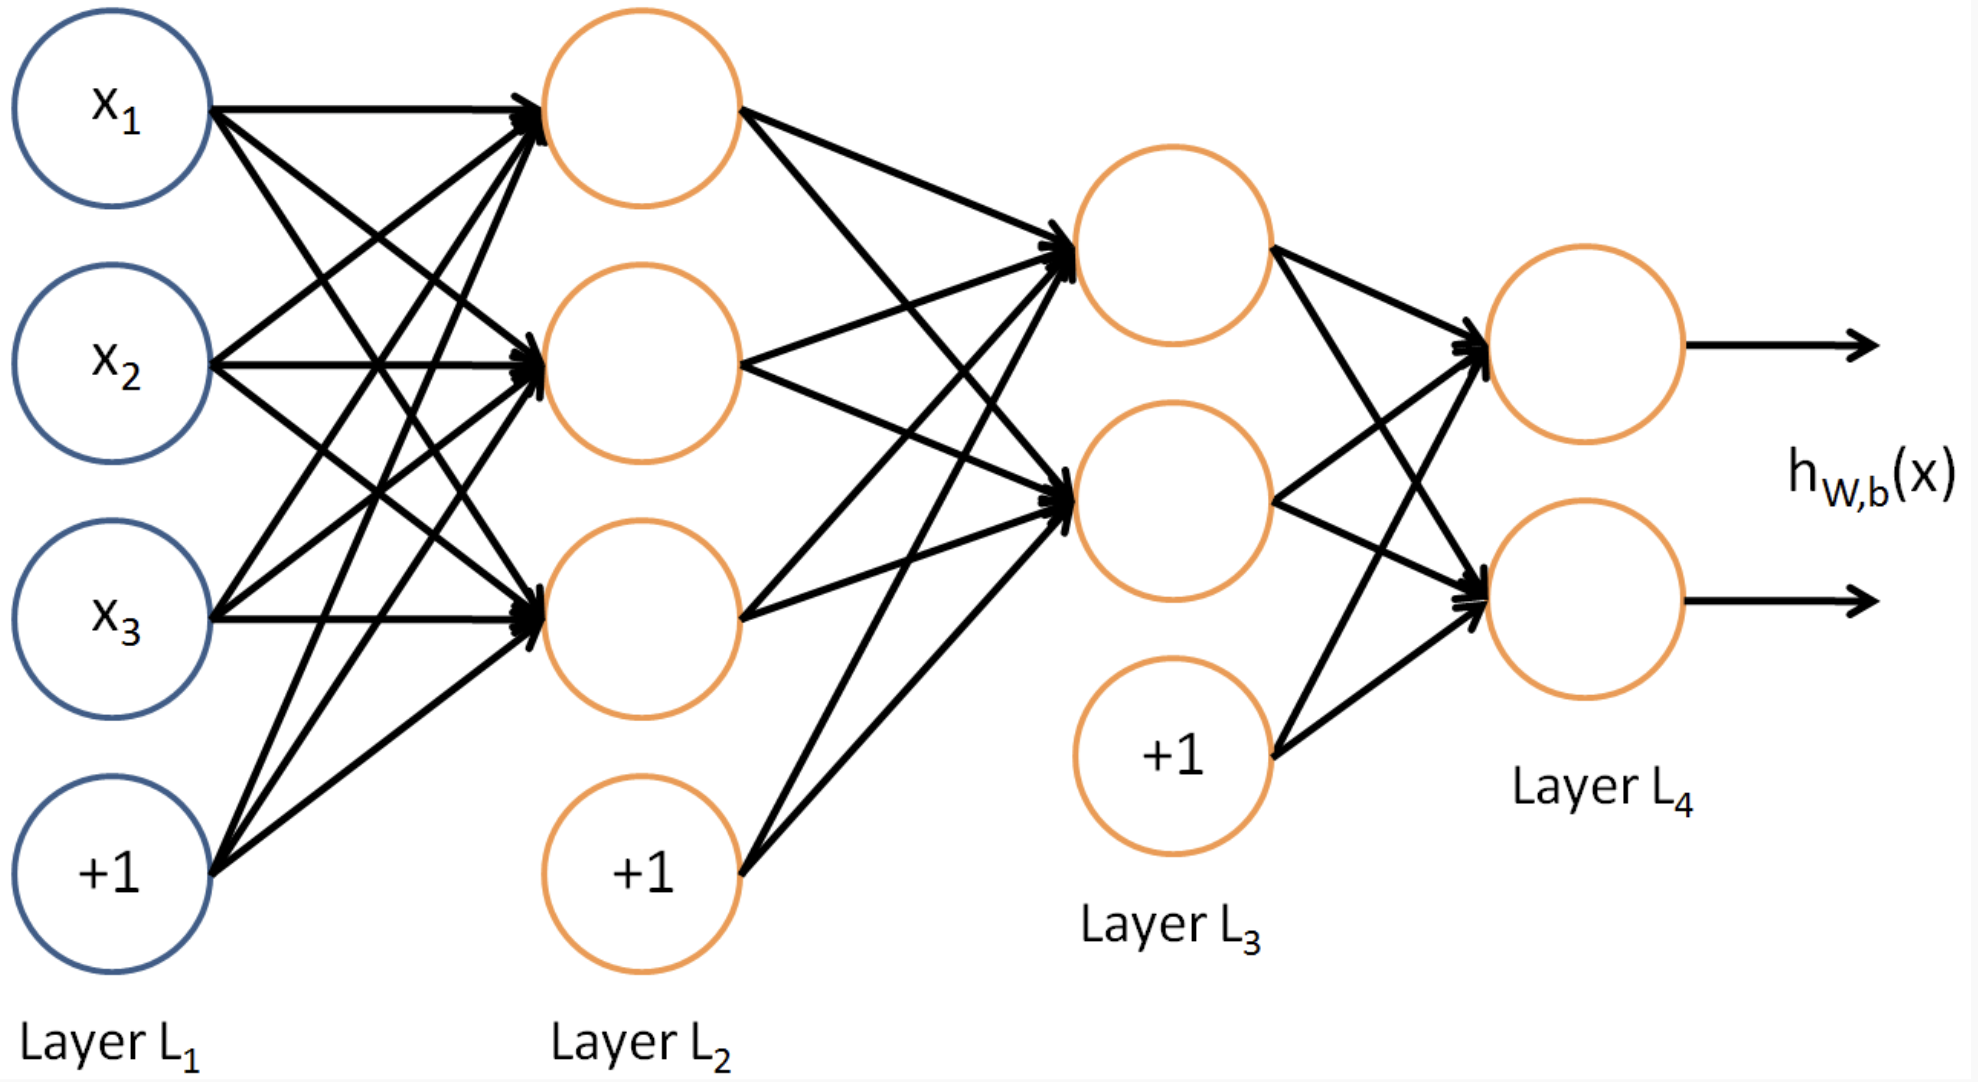
\includegraphics[width=0.6\textwidth]{fotos/43.png}
\caption{Red neuronal con múltiples capas ocultas y múltiples unidades de salida.}
\label{fig:7.4}
\end{figure}

Para entrenar esta red, necesitaríamos ejemplos de entrenamiento $(x^{(i)}, y^{(i)})$ donde $y^{(i)} \in \mathbb{R}^2$. Este tipo de red es útil si hay múltiples salidas que te interesa predecir. Por ejemplo, en una aplicación de diagnóstico médico, el vector $x$ podría proporcionar las características de entrada de un paciente, y las diferentes salidas $y_i$ podrían indicar la presencia o ausencia de diferentes enfermedades. \\

Dependiendo del tipo de problema a afrontar, se toman ciertas consideraciones generales: 
\begin{itemize}
\item Regresión.
\begin{itemize}
\item Una salida por cada variable de salida.
\item La función de salida es generalmente la función identidad.
\item Estandarización de los datos (entradas y salidas), ya que el rango depende de la función de activación.
\end{itemize}
\item Clasificación. 
\begin{itemize}
\item Para clasificación binaria, se utiliza una única unidad de salida y la sigmoide como función de salida.
\item Para una clasificación de $K$ clases, se utilizan $K$ unidades de salida: \textit{encoding} $[1 \; 0 \; 0 \; 0]^T$, $[0 \; 1 \; 0 \; 0]^T$, $[0 \; 0 \; 1 \; 0]^T$, $[0 \; 0 \; 0 \; 1]^T$.
\item La función de salida es generalmente la función \textit{softmax}.
\begin{equation}
f(z_i^{(l)}) = \frac{\exp(z_i^{(l)})}{\sum_{j = 1}^K \exp(z_j^{(l)})}
\end{equation}
\begin{example}
Salida de la función \textit{softmax} para un caso de clasificación de 3 clases: bicicleta, coche y camión.
\begin{table}[H]
\centering
\begin{tabular}{ccccc}
\hline \hline
 & $z_i$ & $\exp(z_i)$ & $f(z_i)$ & Prob. correctas \\ \hline \hline
Bicicleta & $-0.2$ & $0.8$ & $0.2$ (2\%) & $0.00$ \\
Coche & $3.6$ & $36.6$ & $0.75$ (75\%) & $1.00$ \\
Camión & $2.4$ & $11.0$ & $0.23$ (23\%) & $0.00$ \\ \hline 
\end{tabular}
\end{table}
\end{example}
\end{itemize}
\end{itemize}

\section{Funciones de coste o error}

Sea un conjunto de entrenamiento $\{(x^{(1)}, y^{(1)}), \ldots, (x^{(m)}, y^{(m)})\}$. 

\subsection{Logartimo negativo de la verosimilitud}

Intuitivamente, queremos maximizar la probabilidad de verosimilitud sobre los datos de entrenamiento; esto es, cada punto de datos se asume que se genera a partir de la misma distribución de probabilidad
\begin{equation}
\mathcal{P} = \prod_{i = 1}^m p(x_i, y_i) = \prod_{i = 1}^m p(y_i \mid x_i) p(x_i)
\end{equation}

Sin embargo, el producto de probabilidades en poco estable numéricamente (se obtienen valores muy pequeños), por lo que se suele usar el logaritmo negativo de la verosimilitud como función de coste (a minimizar):
\begin{equation}
J = -\log \mathcal{P} = -\sum_{i = 1}^m \log p(y_i \mid x_i) - \log \sum_{i = 1}^m p(x_i) = -\sum_{i = 1}^m \log p(y_i \mid x_i)
\end{equation}

\subsection{Suma del error cuadrático}

\noindent Si se asume que la distribución de los datos es gaussiana,
\begin{equation}
p(y \mid x) = \prod_{i = 1}^m \frac{1}{(2\pi \sigma^2)^{1/2}} \exp\left(-\frac{(h(x_i) - y_i)^2}{2\sigma^2}\right)
\end{equation} 

\noindent se puede usar la suma del error cuadrático como función de coste:
\begin{equation}
J = \frac{1}{2} \sum_{i = 1}^m (h(x_i) - y_i)^2
\end{equation}

\subsection{Entropía cruzada}

\subsubsection{Entropía cruzada binaria}

\noindent Para problemas de clasificación binaria, se puede usar la entropía binaria cruzada como función de coste:
\begin{itemize}
\item Para una sola unidad de salida: $p(\mathcal{C}_1 \mid x_i) = h(x_i)$ y $p(\mathcal{C}_2 \mid x_i) = 1 - h(x_i)$
\item La función de salida es la sigmoide, por lo que se interpreta como una probabilidad.
\end{itemize}

\noindent En caso de tener más de una unidad de salida,
\begin{equation}
p(y_i \mid x_i) = (h(x_i))^y_i (1 - h(x_i))^{1 - y_i}
\end{equation}

\noindent y la función de coste es
\begin{equation}
J = -\sum_{i = 1}^m \left(y_i \log h(x_i) + (1 - y_i) \log (1 - h(x_i))\right)
\end{equation}

Esta función de error es mínima cuando las predicciones del modelo coinciden con las etiquetas reales, esto es $h(x_i) = y_i$. La derivada de esta función respecto a la salida del modelo $h(x_i)$ es
\begin{equation}
\frac{\partial J}{\partial h(x_i)} = \frac{h(x_i) - y_i}{h(x_i)(1 - h(x_i))}
\end{equation}

\subsubsection{Entropía cruzada}

\noindent Para problemas de clasificación multiclase ($K$ clases), con clases mutuamente excluyentes, se tiene que 
\begin{align}
p (\mathcal{C}_k \mid x_i) &= h^k(x_i) \\
p (y_i \mid x_i) &= \prod_{k = 1}^K (h^k(x_i))^{y_i^k}
\end{align}

donde el superíndice $k$ simplemente indica la clase $k$-ésima. La función de coste asociada es 
\begin{equation}
J = -\sum_{i = 1}^m \sum_{k = 1}^K y_i^k \log h^k(x_i)
\end{equation}

En el caso de tener $K$ clases mutuamente no excluyentes, se asume independencia en las categorías, esto es
\begin{equation}
p (y_i \mid x_i) = \prod_{k = 1}^K (h^k(x_i))^{y_i^k} (1 - h^k(x_i))^{1 - y_i^k}
\end{equation}

\noindent y la función de error se escribe como 
\begin{equation}
J = -\sum_{i = 1}^m \sum_{k = 1}^K \left(y_i^k \log h^k(x_i) + (1 - y_i^k) \log (1 - h^k(x_i))\right)
\end{equation}

Ambas funciones de coste tienen un mínimo de error en $h^k(x_i) = y_i^k$. Los valores de salida pasan por una \textit{softmax}, por lo que se interpretan como probabilidades.

\begin{example}
Sean tres clases mutuamente excluyentes: bicicleta, coche y camión. Suponemos que la salida de la función \textit{softmax} es 
\begin{table}[H]
\centering
\begin{tabular}{cc}
\hline \hline
Clase & \textit{softmax} \\ \hline \hline
Bicicleta ($k = 1$) & 0.02 \\
Coche ($k = 2$) & 0.75 \\
Camión ($k = 3$) & 0.23 \\ \hline
\end{tabular}
\end{table}

\noindent La función de coste, al ser clases mutuamente excluyentes, es
\begin{equation}
J = -\sum_{i = 1}^m \sum_{k = 1}^K y_i^k \log h^k(x_i)
\end{equation}

\noindent Así, $J = - (0.0 - 0.29 - 0.0) = 0.29$ ya que  
\begin{itemize}
\item $k = 1$: $0 \cdot \log (0.02) = 0.0$
\item $k = 2$: $1 \cdot \log (0.75) = -0.29$
\item $k = 3$: $0 \cdot \log (0.23) = 0.0$
\end{itemize}

Dependiendo de las probabilidades de salida, se obtiene un valor de error distinto que nos indica cuán bien está clasificando el modelo. Supongamos varios casos:
\begin{table}[H]
\centering
\begin{tabular}{cccl}
\hline \hline
Clase real & \textit{softmax}(h) & $J$ &  \\ \hline \hline
Coche & $\{0.02, \textcolor{green}{0.75}, 0.23\}$ & $0.29$ & Buen clasificador \\
Coche & $\{0.00, \textcolor{green}{1.00}, 0.00\}$ & $0.00$ & Clasificador perfecto \\
Camión & $\{0.00, \textcolor{red}{0.75}, 0.25\}$ & $1.39$ & Mal clasificador \\
Camión & $\{0.00, \textcolor{red}{1.00}, 0.00\}$ & $\gg$ & El peor clasificador posible \\
\end{tabular}
\end{table}
\end{example}